\documentclass[12pt, a4paper, oneside]{article}\usepackage[]{graphicx}\usepackage[]{color}
%% maxwidth is the original width if it is less than linewidth
%% otherwise use linewidth (to make sure the graphics do not exceed the margin)
\makeatletter
\def\maxwidth{ %
  \ifdim\Gin@nat@width>\linewidth
    \linewidth
  \else
    \Gin@nat@width
  \fi
}
\makeatother

\definecolor{fgcolor}{rgb}{0.345, 0.345, 0.345}
\newcommand{\hlnum}[1]{\textcolor[rgb]{0.686,0.059,0.569}{#1}}%
\newcommand{\hlstr}[1]{\textcolor[rgb]{0.192,0.494,0.8}{#1}}%
\newcommand{\hlcom}[1]{\textcolor[rgb]{0.678,0.584,0.686}{\textit{#1}}}%
\newcommand{\hlopt}[1]{\textcolor[rgb]{0,0,0}{#1}}%
\newcommand{\hlstd}[1]{\textcolor[rgb]{0.345,0.345,0.345}{#1}}%
\newcommand{\hlkwa}[1]{\textcolor[rgb]{0.161,0.373,0.58}{\textbf{#1}}}%
\newcommand{\hlkwb}[1]{\textcolor[rgb]{0.69,0.353,0.396}{#1}}%
\newcommand{\hlkwc}[1]{\textcolor[rgb]{0.333,0.667,0.333}{#1}}%
\newcommand{\hlkwd}[1]{\textcolor[rgb]{0.737,0.353,0.396}{\textbf{#1}}}%

\usepackage{framed}
\makeatletter
\newenvironment{kframe}{%
 \def\at@end@of@kframe{}%
 \ifinner\ifhmode%
  \def\at@end@of@kframe{\end{minipage}}%
  \begin{minipage}{\columnwidth}%
 \fi\fi%
 \def\FrameCommand##1{\hskip\@totalleftmargin \hskip-\fboxsep
 \colorbox{shadecolor}{##1}\hskip-\fboxsep
     % There is no \\@totalrightmargin, so:
     \hskip-\linewidth \hskip-\@totalleftmargin \hskip\columnwidth}%
 \MakeFramed {\advance\hsize-\width
   \@totalleftmargin\z@ \linewidth\hsize
   \@setminipage}}%
 {\par\unskip\endMakeFramed%
 \at@end@of@kframe}
\makeatother

\definecolor{shadecolor}{rgb}{.97, .97, .97}
\definecolor{messagecolor}{rgb}{0, 0, 0}
\definecolor{warningcolor}{rgb}{1, 0, 1}
\definecolor{errorcolor}{rgb}{1, 0, 0}
\newenvironment{knitrout}{}{} % an empty environment to be redefined in TeX

\usepackage{alltt} % Paper size, default font size and one-sided paper
%\graphicspath{{./Figures/}} % Specifies the directory where pictures are stored
%\usepackage[dcucite]{harvard}
\usepackage{rotating}
\usepackage{pdflscape}
\usepackage[flushleft]{threeparttable}
\usepackage{multirow}
\usepackage{appendix}
\usepackage[comma, sort&compress]{natbib}
\usepackage{amsmath}
\usepackage{setspace}
\usepackage{appendix}
\usepackage{graphicx}
%\bibliographystyle{plainnat}
\bibliographystyle{agsm}
\usepackage[colorlinks = true, citecolor = blue, linkcolor = blue]{hyperref}
%\hypersetup{urlcolor=blue, colorlinks=true} % Colors hyperlinks in blue - change to black if annoying
%\renewcommand[\harvardurl]{URL: \url}
 \usepackage{listings}
  \usepackage{tikz}
 \usetikzlibrary{arrows,positioning}
 \usepackage{color}
 %\graphicspath{{../Pictures/}}
\definecolor{mygrey}{gray}{0.95}
\lstset{backgroundcolor=\color{mygrey}}
\IfFileExists{upquote.sty}{\usepackage{upquote}}{}
\begin{document}
\title{International Capital Flows and Speculation}
\author{Rob Hayward\footnote{University of Brighton Business School, Lewes Road, Brighton, BN2 4AT; Telephone 01273 642586.  rh49@brighton.ac.uk. }} 
\date{\today}
\maketitle
  \begin{abstract}An SVAR model of the real exchange rate and intentional capital flows reveals that innovations to speculation can cause changes in competitiveness.  Adding measures of speculation to existing models of exchange rates and international capital flows reduces the economic and statistical significance of conventional portfolio flows unless they represent official intervention in the foreign exchange market.   The SVAR method allows a full interaction between the exchange rate and captial flows.  THe results are robust to a number of specifications.  
\end{abstract}

\section{Introduction} 
The rise in gross and net international capital flows that has taken place in the last 20 years has been documented by \citet{PLane2007}, \citet{obstfeldtaylor}, the \citet{BISFX2013} and others. At the same time evidence has accumulated that the link between international capital flows and economic development is not as prominent in practice as it appears to be in theory.  For example, even before the Global Financial Crisis (GFC), \citet{MishkinFinInstab} highlighted the failure of capital to flow from developed to less developed countries as conventional theory would predict; more recently, \citet{HauEquity} review the evidence on the benefits of international financial flows and find it elusive.  

Indeed, international capital flows can have a very disruptive influence.   \citet{CalvoSS},\citet{DornbuschSS} and \citet{KrugmanSS} have investigated the effect of \emph{sudden stops} when capital inflows reverse. The research has expanded to assess the combined influence of the \emph{sudden surge} that proceeds the outflow and to a consideration of the mixture of gross inflows and outflows that affect the balance of payments.  For example, \citet{cavalloSS} create a taxonomy of stops based on the composition of the financial account adjustment and the effect that it has on economic growth, the exchange rate and inflation in the target country.   

The destructive nature of capital flows has renewed interest in capital controls and other means of reducing their influence.  There is evidence from Malaysia, China and Brazil that they can be effective in practice.  Theoetically, \citet{brunnermeier2014international} develop a two-country neoclassical stochastic growth model where banking credit can become excessive because of capital inflows and can disappear quickly when these flows reverse.  Capital controls or macro-prudential measures can improve outcomes. \citet{KatanoCapital} compares the effect of capital controls and perfect capital mobility and finds that the less efficient the financial system the more likely that capital controls will be welfare enhancing. \citet{Korinek2011} makes the case for variable taxation of capital flows on the basis that individual investors do not internalise the increase in aggregate cash risk that individual inflows cause.  He calls for taxes based on the liquidity of the flow-type to price this externality.   

Other evidence suggests that the more short-term and speculative the capital flow, the more disruptive and less beneficial.  \citet{Ozan} finds that for the period 1990 to 2003, a capital inflow that is dominated by private loans and portfolio flows rather than direct investment is more likely to be followed by a sudden stop.   \citet{RazinCap} identify a pecking order in these financial flows with FDI having the least cost in terms of reversal risk; equity flows generally being less prone to stops and reversals; and, debt, particularly with short maturity, being the most dangerous. \citet{RodrickVelasco} study 32 countries through the period 1988 to 1998 and find that those with the highest proportion of debt are the most likely to suffer financial flow reversal and \citet{MontielReinhart} discover that foreign exchange intervention, particularly if sterilised,  can exacerbate the attraction of short-term speculative flows by increasing domestic interest rates and by encouraging the belief that exchange rate stability will be promoted by the central bank.    

There appear to be two major components to speculative currency activity: the a momentum effect and the carry-trade. Each of these can contribute to the cycle of capital surges and capital stops.  Momentum is associated with a gradual building of positive sentiment and an occasional sharp, unexpected reversal of opinion.  The carry trade is tries to take advantage of the failure of Uncovered-Interest-Parity (UIP) to hold.  It generally involves borrowing at relatively low rates in \emph{funding currencies} such as the US dollar, Japanese yen, Swiss franc or euro and using the proceeds to deposit in higher interest rates currencies.  This can cause disruption when large inflows become a constraint on monetary policy and even larger problems when, fearing shock, discrete devaluation of the divestment currency, inflows reverse as traders rush to close their exposed positions. 

Identifying speculative flows has been a challenge due to the scarcity of data.  A standard approach has been to use \citet{BISbanking}. These figures record cross-border banking exposure.  For example, \citet{Bruno2014} model the global liquidity cycle of international banks; \citet{AdamsKaneGlobal} try to assess the relative importance or willingness to lend, the level of liquidity and measures of solvency in determining capital flow.  However, it is impossible using this data to distinguish between bank lending for real business projects and that for speculation in financial markets.  As a rare exception, \citet{Cerutti2014} combine BIS with proprietary data to analyse the flow between international and local banks. 

Exchange rate models that incorporate capital flows are being developed. However, the process has been constrained by missing data and the complexity of the interaction. This paper addresses these issues by broadening the range of capital flows that are included in the model and by using a structural model to fully capture the relationship between capital flow and the exchange rate. In addition to discussing the empirical evidence that underpins the relationship between capital flows and the exchange rate, speculative activity is measured and the effect of exchange rate intervention is assessed.  There are three related contributions:  using SVAR to model international capita flows and the real exchange rate, adding speculation to the capital flow model and identifying the effect of specuilation on competitiveness.   
 The main results are presented in Figure \ref{fig:IRF1} where it is evident that innovations to speculative sentiment and the interest rate spread can have a significant effect on the real exchange rate.  IRF show that a one unit innovation or shock to the S1 series, equal to a ten percentage point change in the net position of speculators relative to the total speculative positions, will have on average, a positive effect of close to 4\% on the real trade-weighted exchange rate over the next eight quarters.  The 95\% confidence intervals, denoted by the red, dashed lines, reveal that it is very likely that there is a positive effect.  For speculative flows that are linked to the interest rate differential, a one-unit or one hundred basis-point improvement in US interest rate advantage tends on average to have an effect of increasing the US real trade-weighted index by about 10\%.  Here there is more uncertainty and there are residual samples when the effect is quite minimal. 

\begin{sidewaysfigure}
\graphicspath{{../Figures2/}}
\centering
\caption{Impulse Response Functions for RTWI for Specification One}
\label{fig:IRF1}
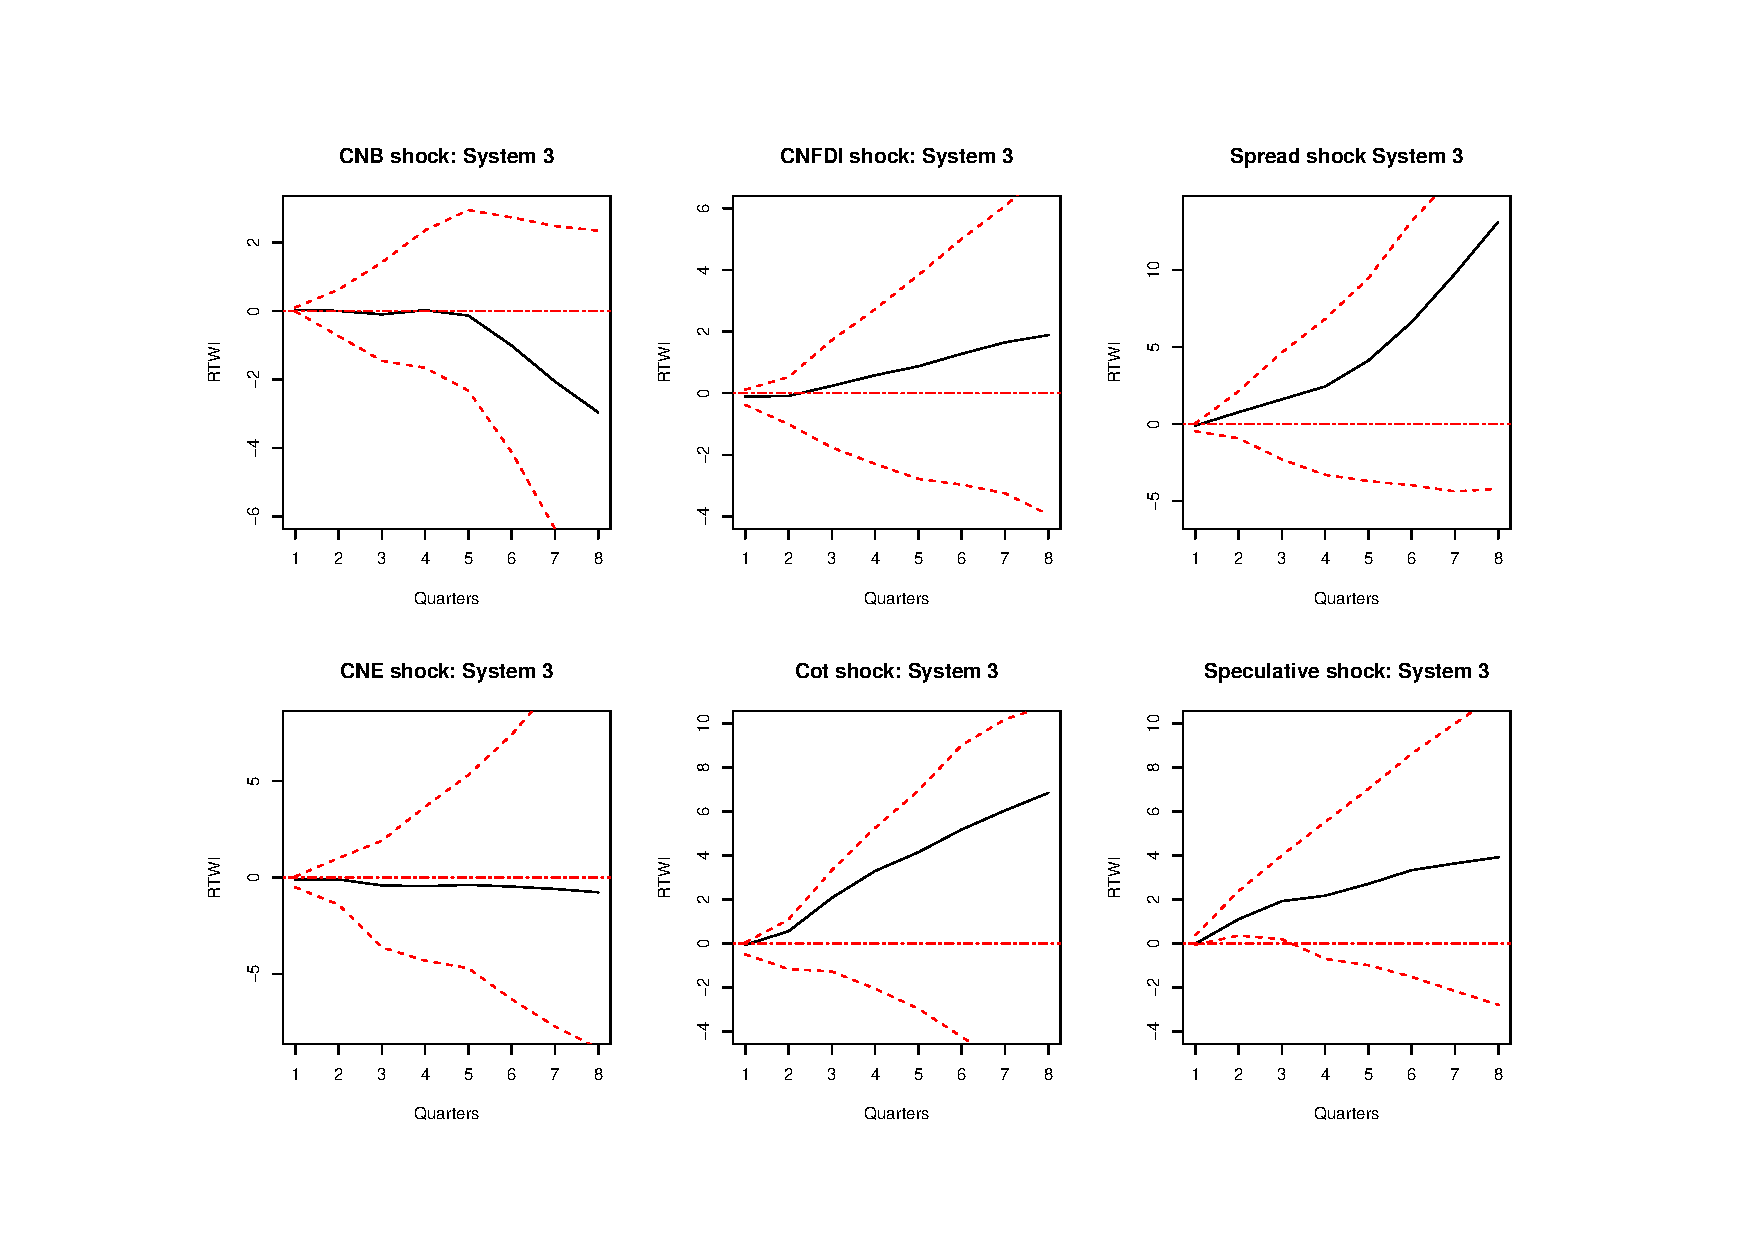
\includegraphics[scale=0.75]{IRF3}
\end{sidewaysfigure}
% does the section on impulse response function fit here? 

For the other major flows, there is a great deal more ambiguity.  The effect of a one-unit increase in the net cumulative bond position relative to GDP (equivalent to about \$35bn at the beginning of 2010) is close to zero over the following four quarters and slightly negative beyond that point.  The impulse response functions show a range of possible outcomes that are centred around zero.  The average effect of an innovation to the net inflow to US equities of one percentage point of GDP or about \$35bn is on average zero but the confidence intervals are wide, suggesting that sometimes the equity inflow is associated with an appreciation of the real exchange rate and sometimes with a depreciation.    The net flow associated with foreign direct investment is very similar to that of equities, but slightly more positive.  

The action of overseas central banks is also of interest.  A one unit exceptional increase in central bank net holding of treasuries, almost certainly a consequence of foreign exchange intervention to purchase US dollars with a sale of their domestic currency, is associated with an average positive move of 4\% over the next four quarters. It appears that this intervention in the foreign exchange market is successful in the short-term on the assumption that it takes place because of initial US dollar weakness. The width of the confidence intervals indicates that there are occasions when the capital flow associated with central bank intervention does not have the desired influence and weakness in the US real trade-weighted index continues.   

The overall impression is one where speculation, whether sentiment-orientated or part of a carry-trade activity, has a much more consistent and significant effect on the real exchange rate than the other capital flows.  This effect is not as short-term as is often envisaged, it continues to have an influence for several quarters. It is also clear that central bank intervention can affect the level of the exchange rate. 

The rest of this paper is oganised as follows..

\section{Capital flow and the exchange rate}
Standard models of exchange rates have put the emphasis on the goods market. \citet{OandR} provide an overview of the most widely used open-economy macro model that concentrates on relative prices and the adjustment via the current account.  International financial markets are complete and therefore act as an automatic facilitator of any current account imbalance.  International financial flows can be incorporated so that there are adjustments to country-specific exogenous innovations like productivity shocks through inter-temporal transfers.  This involves capital flows and changes in the stock of net international investments. See \citet{obstfeld2000new}, \citet{OandRedux} and \citet{lane2001new} for a survey of the literature. 

The financial account and the role that portfolio adjustment plays in the evolution of exchange rates has generally received less attention.  However, \citet{Branson1971} presents a model of international capital flows. This is a stock, equilibrium, reduced-form model where changes in capital flows depend on changes in relative interest rates and changes in the the size of the overall stock of savings.  \citet{Kouri1974International} develop a Portfolio Equilibrium model and extend Branson by adding the traditional monetary approach to the balance of payments. Capital flows are therefore affected by the domestic excess demand for money and interest rates are endogenous.   
  
More recently, \citet{brookscapital} assess the ability of portfolio and foreign direct investment to track movements in the US dollar against the Yen and the Euro. They look at the relationship between the excess returns for the US market relative to that of the Euro area as an explanation for the capital flow and exchange rate changes. A standard linear empirical exchange rate model presented by \citet{Siourounis2004Capital}, he finds that net US equity purchase has a stable and consistent impact on UK, German and Swiss exchange rates, but that net purchase of US or overseas bonds have no effect.   A vector auto-regression (VAR) is employed and impulse response functions (IRF) and variance decomposition are estimated to help understand the relative importance of difference types of capital flow.  
  
\citet{HauEquity} derive exchange rates from the financial account of the balance of payments where there is less than fully elastic supply of currency.  Net demand for overseas equities will drive the exchange rate in an extension of the microstructure approach.  This is an increasingly familiar approach (see \citet{Geliman}). However, while in the microstructure literature \citet{Evans2002Order}, \citet{Lyons1995Microstructure} and \citet{rime2010exchange} explain movements in currency with knowledge about market-maker and dealer orders, here the movement of international capital is the fulcrum of adjustment.

On the assumption that all dividends are repatriated, Hau and Rey express the capital outflow for the equity market $(Q_t)$ as

\begin{equation}
dQ_t = E_tK_t^{h*}D_t^hdt - K_t^fD_t^fdt + dK_t^fP_t^f - E_tdK_t^{h*}P_t^h
\end{equation}

where $E_t$ is the exchange rate at time $t$ expressed as foreign units of domestic currency; equity holding at time $t$ are $K_t$, divided between home equities $K_t^h$ and foreign $K_t^f$; $D^h_t$ and $D^f_t$ are the home and overseas dividend payments; $P_t^h$ and $P_t^f$ are the home and overseas stock prices respectively.   

The foreign exchange market is assumed to be incomplete and the exchange rate follows a \emph{Ornstein-Uhlenbeck process}\footnote{This is a mean-reverting process that has the following stochastic difference equation: $dx_t = \theta(\mu - x_t)dt + \sigma dW_t$ where $W_t$ is the \emph{Wiener process} and $\theta$ , $\mu$ and $\sigma > 0$.} with a long-run equilibrium value of the exchange rate at $\bar{E}$ and a rate of mean reversion of $\alpha$. The supply of currency to satisfy the imbalance of demand caused by net capital flows to overseas equity markets is 

\begin{equation}
Q^s = -\kappa(E_t - \bar{E})
\end{equation}

Therefore, excess net demand for overseas equities will cause an appreciation of the overseas currency as a means of inducing risk-averse market-makers and speculators to hold more domestic currency.  Speculators facilitate the decisions of equity investors through price concession. This is consistent with the Keynes-Hicks model of speculations ( \citet{KeynesHedge} and \citet{HicksHedge}).   
%Note 20 closes the model.  The flow is offset by a movement of currency that is absorbed by the central bank. Is this different from the financial system absorbing or completing the model? 

% Can this be used at some ponit. The two extremes of the Hau Rau model. This is a world half-way between financial autarchy where investors hold only domestic assets and where there is complete risk sharing through the use of foreign exchange derivatives and domestic and foreign equities are held in proportion to their capitalisation (50:50 in the model). 
 
Similarly, \citet{Blanchardint} try to determine whether central bank intervention in the foreign exchange market can be successful when there are no monetary or signalling effects.  The model here is determined much more by short-term speculation than relatively high interest rates. 

\begin{equation}
GPKI_{j,t} - GPKO_{j,t} + FXI_{j,t} +CA_{j,t} = 0
\end{equation}

where GPKI is gross private capital inflow and GPKO is gross capital outflow, FXI is official foreign exchange intervention and CA is the current account position. 

Each of the main components is determined by 

\begin{subequations}
\begin{equation}
GPKI_{j,t} = \alpha (i_{j,t} - i^*_t - e_{j,t} +Ee_{j, t+1}) + z_t
\end{equation}
\begin{equation}
GPKO_{j,t} = -\beta (i_{j,t} - i^*_t - e_{j,t} + Ee_{j,t+1}) + \rho z_t
\end{equation}
\end{subequations}

where $i_{j,t}$ is the domestic interest rate, $i^*_t$ is the overseas interest rate, $e_{j,t}$ is the current exchange rate, $e_{j,t}$ is the exchange rate in the next period and $z_t$ is a set of exogenous variables that drive capital flows (such as risk appetite). 

The current account is assumed to be a linear function of the exchange rate so that, 

\begin{equation}
CA_t = -\gamma e_{j,t}
\end{equation} 

with $\gamma \leq 0$.  

Parameters $\alpha$ and $\beta$ are parameters that measure the sensitivity of capital flows to return differentials. These are expected to be positive.   

The parameter $\rho$ measures how sensitive domestic investors are to global financial shocks relative to international (normalised to one). In general it seems that $\rho \leq 0$ as repatriation in the event of an increase in risk aversion means that a reduction in gross outflow offset the effect of a reduction in gross inflow.  

\section{Methodological issues}
Two methodological issues are to be addressed: the set of explanatory variables and the problem of endogeneity. There are a very wide range of economic variables that can be expected to affect the exchange rates.   Most of the models discuss above concentrate on the equity or bond flows, leaving no room for the influence of short-term activity.  The statistical difficulties that emerge when trying to estimate parameters when there is feedback from the dependent variable onto explanatory variables was an important part of the criticism of the Branson model.\footnote{See \citet{Branson1968} and \citet{Branson1971}.}  \citet{Kouri1974International} show that a linear regression of capital flows on interest rate differentials will systematically under-estimate the sensitivity of capital flows. The \citet{brookscapital} model suffers in the same way from being reduced form.   

Vector Auto Regression (VAR) is one way of dealing with the issue of endogeneity.  The method was initially suggested by \citet{Sims1980Macroeconomics}.  An overview of developments and extensions can be found in \citet{lutkepohlvar} and \citet{Hamilton}.  The essence of the VAR is to set up a system that is made up of all the important variables, assume that they are endogenous and add significant lags to remove any serial correlation from the equation residuals.   The variables used here are cumulative net equity flows, net bond flows, net foreign direct investment, net official purchase and two variable for speculative activity. The cumulative flows produces a stock of international financial assets so changes in these stocks are related to changes in the real exchange rate.  

The \emph{primitive} version of the VAR is presented in Equation \ref{transitionvar} 

\begin{equation}\label{transitionvar}
Bx_{t}=\Gamma_{0}+\Gamma_{1}x_{t-1}+\epsilon_{t}
\end{equation}

where $x_t$ is a vector of the endogenous variables, $\epsilon_t$ is a matrix of innovations with the assumption that non-diagonal covariance elements are zero and normally distributed with a constant variance\footnote{Though the independence assumption appears quite onerous, it should be remembered that this is independence of innovation.  It does not mean that there is no relationship between the two variables ($x$ and $y$ here). A shock to either variable will have an effect on the other via the contemporaneous relationship (which is the matrix $B$ in Equation \ref{transitionvar}.}, $\Gamma_0$ and $\Gamma_1$ are parameters to be estimated, and $B$ is a matrix of contemporaneous correlations to be estimated. In the interest of clarity, the exogenous variables are not included.  

To remove the endogeneity, the structural or primitive equations can be transformed so that coefficients can be estimated without the fear of bias. This is done by Multiplying through by $B^{-1}$ will give the \emph{standard form of the VAR}

\begin{equation}\label{standardvar}
x_t=A_0+A_1x_{t-1}+e_t
\end{equation}

Now the equations are in reduced form.  It has been that the ordinary-least-squares estimator is the equivalent to the Maximum Likelihood Estimator (MLE). See \citet[p. 293]{Hamilton} for proof.  However, though the model can be estimated with ease, because of the transformation that has been undertaken, the coefficients that are of interesting in the structural model have been transformed. $A_0=B^{-1}\Gamma_0$, $A_1=B^{-1}\Gamma_1$ and $e_t=B^{-1}\epsilon_t$. Some method must be established to uncover the structural parameters.  As there are seven variables twenty one restrictions are required for identification.  In general, $K(K-1)/2$ restrictions will be required, where K is the number of endogenous  variables in the VAR.

In this paper a structural model of international capital flows and the real exchange rate based on a downward sloping demand  curve that will finance capital movements.  However, here the financing capital flows are extended to include short-term speculative flows from sentiment and relative interest rates. The former uses the short-term positions of speculators in the foreign exchange futures market while the latter uses the interest rate differential. A Structural Vector Autoregressive (SVAR) model addresses the issue of endogeneity as in \citet{Siourounis2004Capital} with plausible restrictions added for identification.  Impulse Repose Functions (IRF) show that innovations to speculative activity drive the US real exchange rate, while innovations to FDI and net equity flow do not have a standard effect.  Innovations to net bond flows are only significant when the sub-category of official bond purchase are used.  These are the flows associated with the intervention of central banks in the foreign exchange market.  
The paper provides additional support to the evidence that international capital flows can drive the real exchange rate, it narrows down this effect to the more speculative activity and it provides some evidence that official intervention in the foreign exchange market to counter speculative activity can be beneficial.  The rest of the paper is organised as follows:  Section \ref{secref:3} presents the model; Section \ref{secref:4} outlines the results and Section \ref{secref:5} concludes. 

\subsection{Identification}\label{secref:ident}
There are a wide variety of methods that can be used to restrict the equation for identification.   \citet{Siourounis2004Capital} uses a relatively simple and common adjustment of the B matrix from Equation \ref{transitionvar} to set all the lower-triangle elements to zero.  The disadvantage of this is that the estimated values of the contemporaneous coefficients will be determined in part by the order that the variables are included in the VAR (see \citet[pp303-311]{EndersTS} for  a full discussion).  The Sims-Bernanke approach, to use economic theory to place restrictions on some of the parameters, is adopted here and compared to the naive model. In assessing the relative importance of fiscal and monetary policy in economic activity,  \citet{Sims1986} proposed a six-variable VAR including factors like GNP, money supply, interest rates, inflation, investment and unemployment and made 17 restrictions so that the system was \emph{over-identified}. Similarly,  \citet{Bernanke1986} made a number of explicit restrictions to support his assertion that the relationship between money and income is intermediated by credit rather than being the result of money illusion or causality running from income to money.  

For $b_t$ cumulative net bond flow, $e_t$ cumulative net equity flow, $i_t$ cumulative net foreign direct investment flow, $re_t$ is the real trade-weighted exchange rate, $cb_t$ is central bank bond purchase, $r$ is the short-term interest rate spread and $s_t$ is speculative activity.  

The system of equations 
\begin{equation}
  b_t = \xi_{be}e_t + \xi_{br} r_t + \varepsilon_{b,t}
\end{equation}

\begin{equation}
e_t = \xi_{ee} b_t + \xi_{ei} i_t + \xi_{ere} re_t + \xi_{es} s_t + \varepsilon_{e,t}
\end{equation}

\begin{equation}
i_t = \xi_{ie} e_t + \xi_{ire} re_t + \varepsilon_{i, t}
\end{equation}

\begin{equation}
cb_t = \xi_{cbre} re_t + \xi_{cbs} s_t + \varepsilon_{cd,t}
\end{equation}

\begin{equation}
re_t = \xi_{ree} e_t + \xi_{rei} i_t + \xi_{recb} + cd_t + \xi_{rer} r_t + \xi_{res} s_t + \varepsilon_{re, t}
\end{equation}

\begin{equation}
r_t = \xi_{rb} b_t + \xi_{rre} re_t + \varepsilon_{r, t}
\end{equation}

\begin{equation}
s_t = \xi_{se} e_t + \xi_{scb} cd_t + \xi_{sre} re_t + \varepsilon_{s, t}
\end{equation}

The system to be estimated is of the form
\begin{bmatrix}
1 & \xi_{be} & 0 & 0 & 0 & \xi_{bs} & 0 \\ 
\xi_{eb} & 1 &  \xi_{ei} & 0 & \xi_{eer} & 0 & \xi_{es} \\
0 & \xi_{ie} & 1 & 0 & \xi_{ire} & 0 & 0 \\
\xi_{cbb} & 0 & 0 & 1 & \xi_{cbre} & 0 & \xi_{cbs}\\
0 & xi_{ree} & \xi_{rei} & \xi_{recb} & 1 & \xi_{rei} & \xi_{res}\\
\xi_{sb} & 0 & 0 & 0 & xi_{sre} & 1 & 0\\
0 & \xi_{se} & 0 & \xi_{scb} & \xi_{sre} & 0 & 1
\end{bmatrix}

\[
\begin{bmatrix}
b\\
e\\
i\\
cb\\
re\\
i\\
s
\end{bmatrix}

= 

\begin{bmatrix}
\varepsilon_{b,t}\\
\varepsilon_{e,t}\\
\varepsilon_{i, t}\\
\varepsilon_{cb,t}\\
\varepslon_{re, t}\\
\varepsilon_{i, t}\\
\varepsilon_{s, t}
\end{bmatrix}



\begin{threeparttable}
\caption{SVAR Restrictions}
\begin{tabular}{p{3cm} rrrrrrrrr}  
  \hline
 &  CNB & CNE & CNFDI & COT & RTWI & SPREAD & S1 \\ 
  \hline
  CNB & 1 & NA & 0a & 0b & 0c & NA & 0d\\ 
  CNE & NA & 1 & NA & 0e & NA & 0f & NA\\ 
  CNFDI & 0g & NA & 1 & 0h & NA & 0i & 0j\\ 
  COT & NA & 0k & 0l & 1 & NA & 0m & NA \\ 
   RTWI & 0n & NA & NA & NA & 1 & NA & NA\\ 
  SPREAD & NA & 0p & 0q & 0r & NA & 1 & 0s\\ 
  S1 & 0t & NA & 0u & NA & NA & 0v & 1\\ 
   \hline
\end{tabular}
\label{tabref:svar1}
\begin{tablenotes}
\small
\item The table shows the individual equations in the VAR and the restrictions that are placed on some of the coefficients to identify the system.  Reading across the page, the first row reads CNB as the dependent variable, NA for CNE meaning that this coefficient can be estimated, there is a zero restriction placed on CNFDI and the letter identifies the explanation for the restriction in the paragraph below.  
\end{tablenotes}
\end{threeparttable}  

The following are the explanations for the twenty-one restrictions that are imposed on the exchange rate-capital flow model.  Note that these are contemporaneous restrictions (same quarter), a lagged effect is still allowed.  The equations are read across rows, with the dependent variable normalised to unity, coefficients on independent variables that are to be estimated are labelled "NA" in Table \ref{tabref:svar1}, and the zero restrictions are labelled alphabetically.  The matrix does not have to be symmetric; for example, a change in cumulative net foreign direct investment to GDP (CNFDI) may affect speculative sentiment in the current quarter, as the confidence expressed by international investors may encourage speculative activity, but that does not mean that an increase in speculative sentiment has to affect CNFDI which may be expected to be influenced by factors that are more long-term or fundamental in their nature.    Table \ref{tabref:svar1} is the equivalent of a seven by seven B matrix in Equation \ref{transitionvar}.   

Reading across the row for each equation in turn. The cumulative net bond equation (CNB) has a one-to-one relationship to itself; is restricted by imposing a coefficient of zero on the influence of foreign direct investment (a); cumulative official treasuries (b), the real exchange rate (c) and sentiment (d).  Though the exchange rate and speculative sentiment could be expected to be related to an increase net bond flows, it seems more likely that this would happen at the short end of the yield curve (and therefore would be better captured by the measures of short-term speculative activity, which is allowed) and, as noted in \citet{HauEquity}, most of the international bond flows appear to be hedged against foreign exchange gains and losses.    The cumulative net equity equation is restricted only at the cumulative official treasuries (e) and the interest rate spread (f).  Lower relative rates could inspire a more positive attitude towards corporate profits, but rate changes could just as likely be a response to broad-based economic weakness that would not be conducive to profitability. The restrictions on the FDI equation are on bond flows (g), official treasuries (h), the interest rate spread (i) and sentiment (j).  As foreign direct investment is assumed to be a more long-term commitment, it seems likely that short-term relationship with other variables will be negligible; the longer term coefficients can play a more prominent role.   The flow of Official Treasuries (COT) is most likely to be a response to an appreciation of the US dollar and therefore should not be significantly affected by things like equity (k) and FDI (l) flows, unless indirectly.  The real exchange rate is allowed to be immediately influenced by all the other variables outside of net bond flows (n).  The interest-rate spread, which presumably is largely a function of central bank policy, is restricted against net equity (p), net FDI (q), official purchase (r) and sentiment (s).  The exchange rate and net bond flows are allowed to have some influence as the exchange rate may be a policy trigger and bond flows may be affected by expected changes in short-term interest rates.  Finally, the sentiment equation is restricted on bonds (t), FDI (u) and the spread (v), but can vary with equity and the exchange rate.  This allows for some positive spillover from more optimistic attitudes towards the economy, which may affect the flow of money to the stock market or into real investments.   It can account for positive feedback from a change in the value of the exchange rate to speculative sentiment, thereby allowing positive momentum. 
It is possible to argue about some of the restrictions that have been imposed here.  However, at least the restrictions are out in the open, can be debated and can be assessed against the available data evidence.  This marks an improvement on the \emph{ad hoc} or \emph{naive} methods use by \citet{Siourounis2004Capital}.  It is  of course possible to run the model, assess the outcome and then make adjustments to the restrictions.  However, this would increase the risk of \emph{data mining} or \emph{over-fitting} and it is not done here.  Nonetheless, as a robustness check, three alternative specifications are assessed:  the first is one that is restricted by setting the lower triangle of matrix B to zero (Specification Two); the second takes a random ordering of the variables with the same lower triangle restriction noted above (Specification Three); the preferred version uses the structural restrictions noted above (Specification One).  The fact that all three methods give similar results, inspires confidence that the outcome is not just a function of the ordering of the variables or the assumptions that have been made to identify the coefficients.   

\section{Results}\label{secref:4}
Once the model has been established, it can be used to assess how variables in the system interact.  This is most usually done by creating \emph{Impulse Response Functions} (IRF).  These are the graphical representations of the effect of a shock or innovation on one part of the system to any other variable.   The \emph{Wold moving average representation} is used to transform a stable autoregressive process into one that is moving average.   See \citep[p. 17]{HarveyTSM}, \citep[pp. 64 - 70]{Hamilton} or \citep[pp. 307-311]{EndersTS} for full details. 
   
Starting from the standard VAR representation of Equation \ref{standardvar}, 

\begin{equation}
x_t=A_0+A_1x_{t-1}+e_t
\end{equation}

by iterating backwards and using the stability assumption, this becomes  

\begin{equation}
x_t=\mu + \sum_{i=0}^{\infty} A_i^i e_{t-i}
\end{equation}

Where $\mu$ is the mean level of the vector $x$. 

The identification discussed in Section \ref{secref:ident} is now used to uncover the structural parameters. In this case, the identification requires that $A_1$ be replaced by the $B^{-1}A_1$.  Which for a two-variable case would be 

\begin{equation}
x_t=\mu + \sum_{i=0}^{\infty} \Phi_i \varepsilon_{t-i}
\end{equation}

when

\begin{equation}
\Phi_i=\frac{A_1^i}{1 - b_{12}b_{21}}
\begin{bmatrix} 1 & -b_{12} \\ -b_{21} & 1 
\end{bmatrix} 
\end{equation}

The IRF will show the average effect that is expected from a shock to one of the endogenous variables given the estimated parameters.  However, the parameters are estimated with some imprecision and therefore it is usual to also draw some confidence intervals around the path to show the nature of this imprecision. There are two methods for constructing the confidence intervals.  The first is to assume that the error in estimating the coefficients of the system has a particular distribution and then use estimates of the parameters of that distribution to find confidence levels.  However, with multicollinearity of the VAR, it is better to use the underlying data to assess the precision of the IRFs by using the \emph{bootstrap method}.  

In this case, the \emph{residual bootstrap} is used.  This involves using a random draw of the residuals from the estimated system, calculating estimated values of the endogenous variables and then re-estimating the coefficients of the system before calculating the IRF.   If this is done 100 times, the empirical distribution can be used to identify the central 95\% (or any other level of precision that is required) of the estimates and use this to define the confidence intervals.  

\section{Robusness of model}
The preferred model, according to the range of information and diagnostics is the one that does not include the current account, has four lags and uses the three dummy variables as well as the S1 and SPREAD2 measures of sentiment and interest rates.  A model with a linear trend and a constant is the one that best fit the data.  It reveals that the system is stable as the roots of the autoregressive coefficients are all within the unit circle.    
 
%it was [h!] now
\begin{figure}
\graphicspath{{../Figures2/}}
\centering
\caption{Cumulative capital flows and USD}
\label{figref:ts}
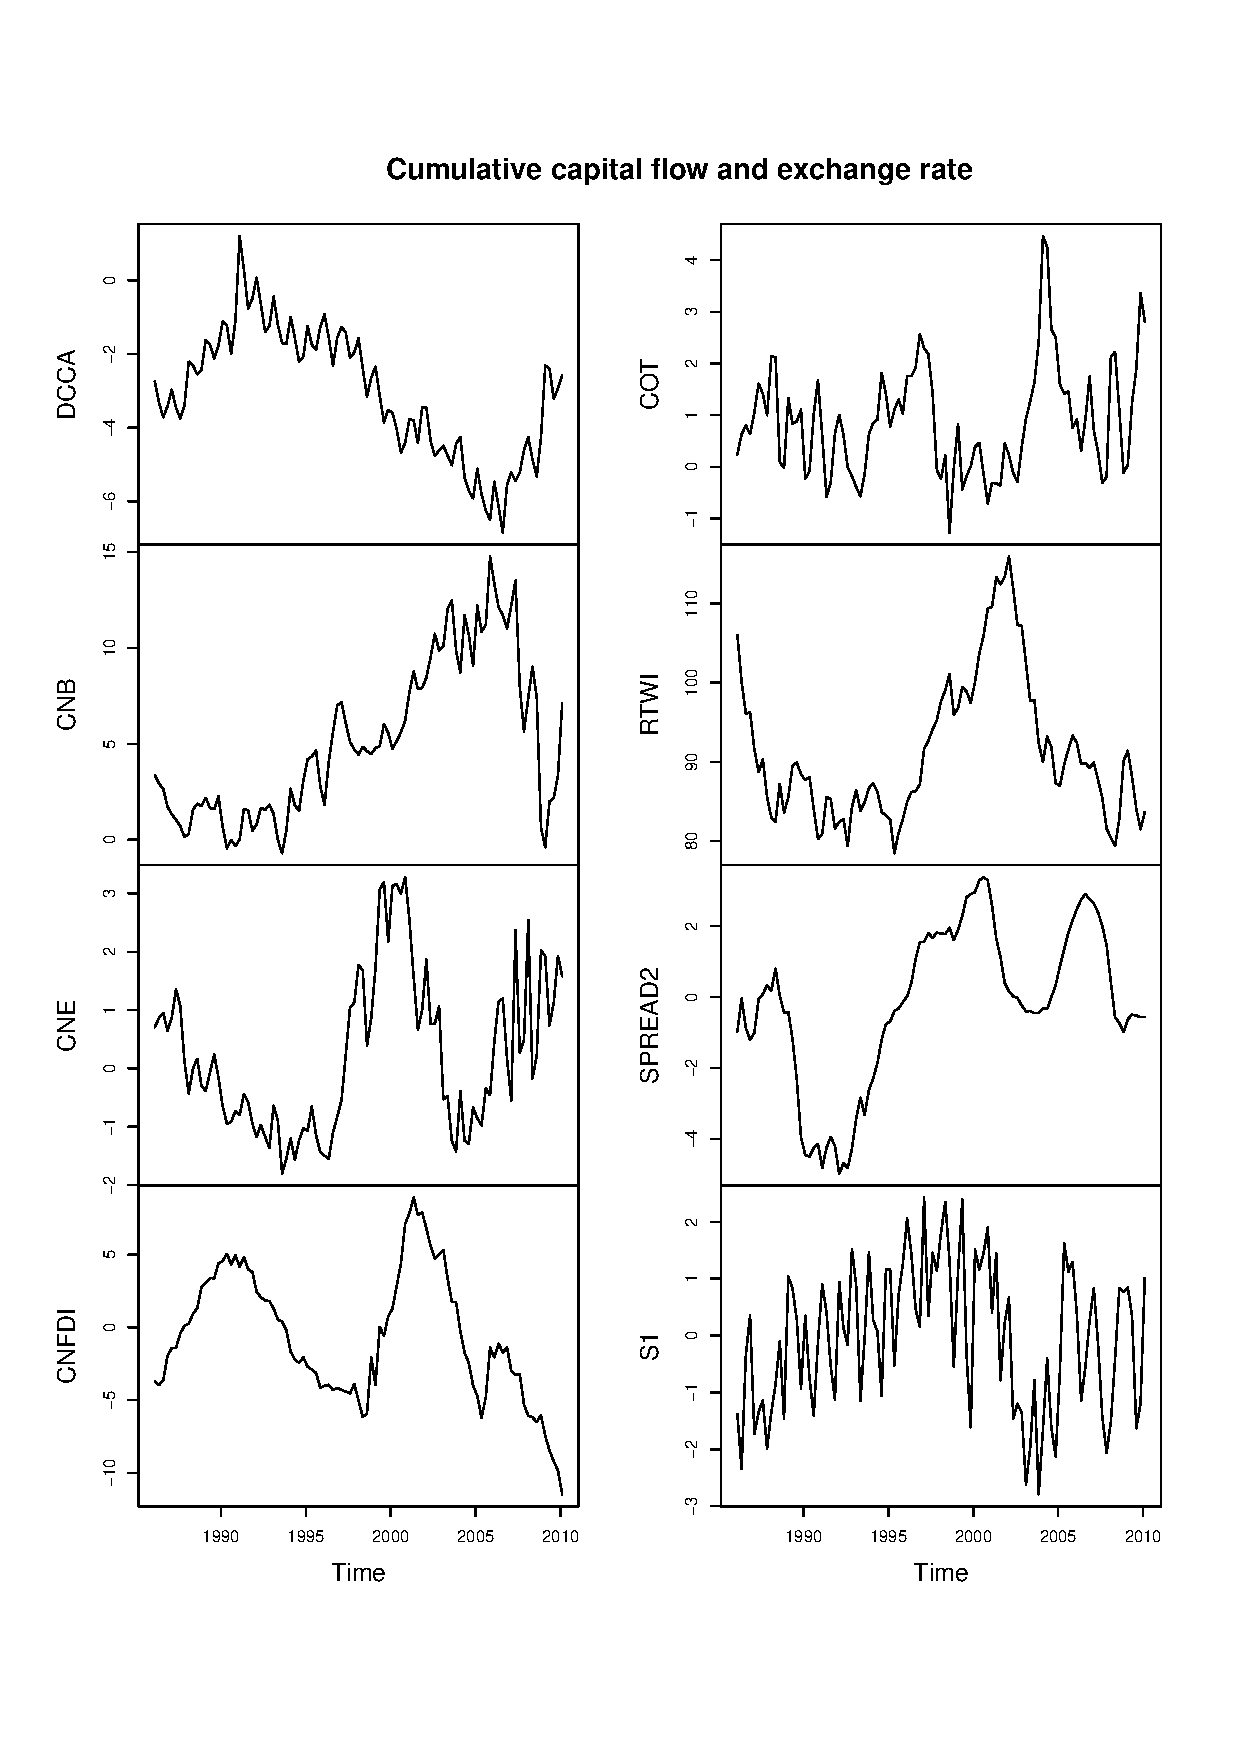
\includegraphics[scale=0.65]{ts}
\end{figure}\label{fig:timeseries}

Figure \ref{fig:timeseries} also shows the significant changes that have taken place in the stock of international financial assets during the period under study.  A number of these warrant more attention.  For example, the scale of the fluctuation in net bond flows becomes apparent.   Cumulative net bond flows increase steadily through the period from 1995 from a fairly flat position to reach a peak of close to 15 percent of GDP at the eve of the financial crisis.  With a nominal GDP of \$3.5trillion in the first quarter of 2010, this is a net increase of around \$500bn in the space of 10 years. 

Exogenous variables can be added to the VAR. These could include an intercept and drift, as used here, as well as seasonal dummies or dummies to account for structural breaks.  There are three exogenous dummy variables that cover periods of unusual activity.  The first dummy (D1) runs from the third quarter of 1986 to the first quarter of 1988.  This is an extreme move in the variable SPREAD1 caused by a sharp movement in Mexican interest rates. The second dummy (D2) covers the period from the second quarter of 1994 to the second quarter of 1995 to encompass a significant increase in US interest rates and the exceptional international outflows from the US bond market.   The third dummy (D3) runs from the third quarter of 2007 to the end of 2008 and represents the disturbance caused by the GFC. 
%%There are also suggestions that the relationship between the exchange rate and the currency have changed over time.  \citet{HauEquity} find a change in relationship in 1994 and 2002;  \citet{Siourounis2004Capital} splits the data into two perilds; before and after 1994.  Also a break at 2002.  Hau and Rey report that the relationship between equity flows and the exchange rate has become stronger. Check these findings. 

%A transfer function of permanent dummy is used to account for a structural shift in the model in 1994 and 2002.  These dummies appear to be important for some of the equations and improve the fit very slightlty (based on AIC and Log Likelihood statistics).  It is possible to check for structural breaks at points like the introduction of the North American Free Trade Agreement (NAFTA) in 1995, the introduction of the Euro in 1999 or September 11.  This would also be one way to deal with the real risk of parameter instability. \section{Roubstness}

A transfer function could also be used to account for a structural shift in the model at some point.  In this case, rather than turning the dummy on for the period of disturbance and then off again when the usual circumstances have come to an end, the transfer function is maintained.  There are no obvious breakpoints that would suggest a clear chance of a structural change.  However, it is possible to check for structural breaks at points like the introduction of the North American Free Trade Agreement (NAFTA) in 1995, the introduction of the Euro in 1999 or September 11.  This would also be one way to deal with the real risk of parameter instability. 

% the changing nature of capital flows may also be addressed. This is something that is assessed in Hau and Rey and in Siourounis. They have a break point at 2004.  Does the model change at this date?  Has speculation become more signficant?  

\begin{sidewaysfigure}
\graphicspath{{../Figures2/}}
\centering
\caption{Impulse Response Functions for RTWI for Specification Two}
\label{fig:IRF2}  
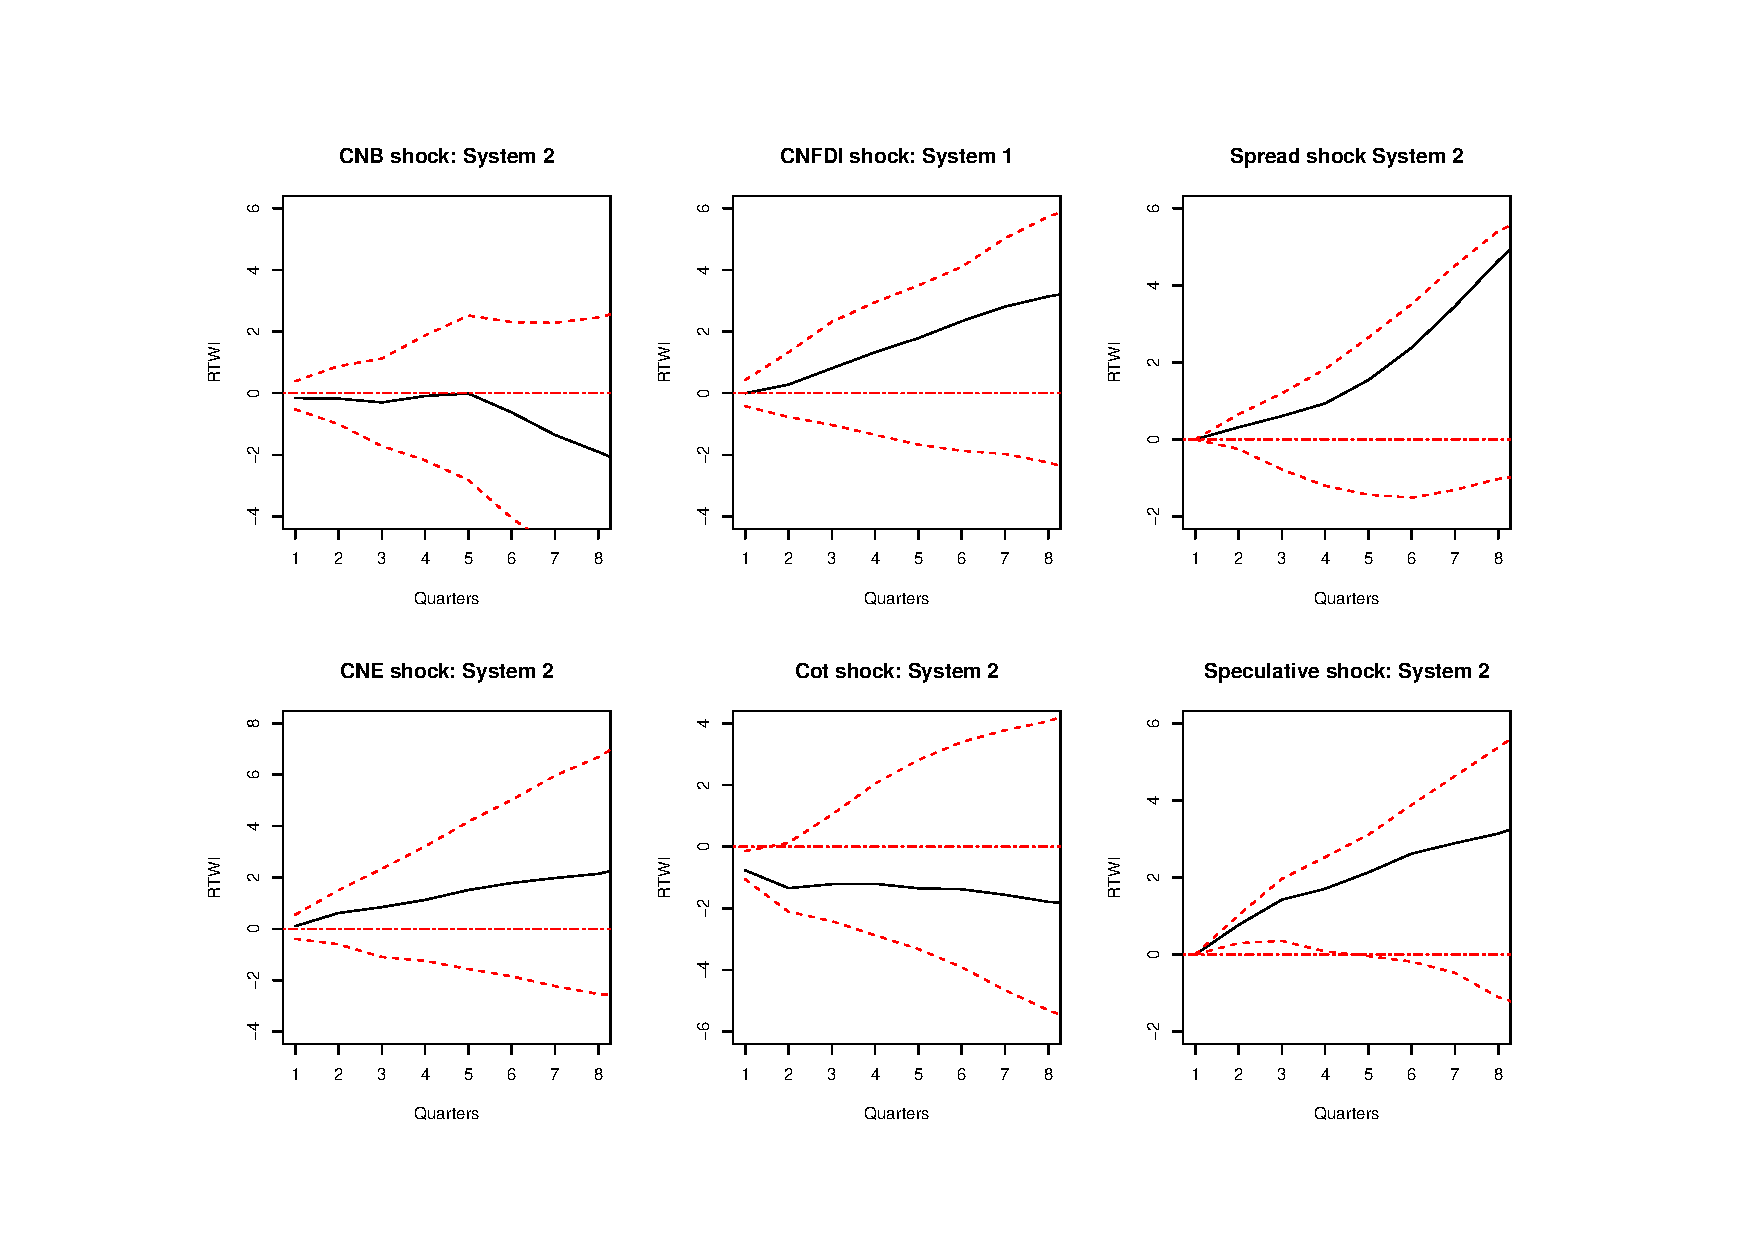
\includegraphics[scale=0.75]{IRF1}
\end{sidewaysfigure}


\begin{sidewaysfigure}
\graphicspath{{../Figures2/}}
\centering
\caption{Impulse Response Functions for RTWI for Specification Two}
\label{fig:IRF3}  
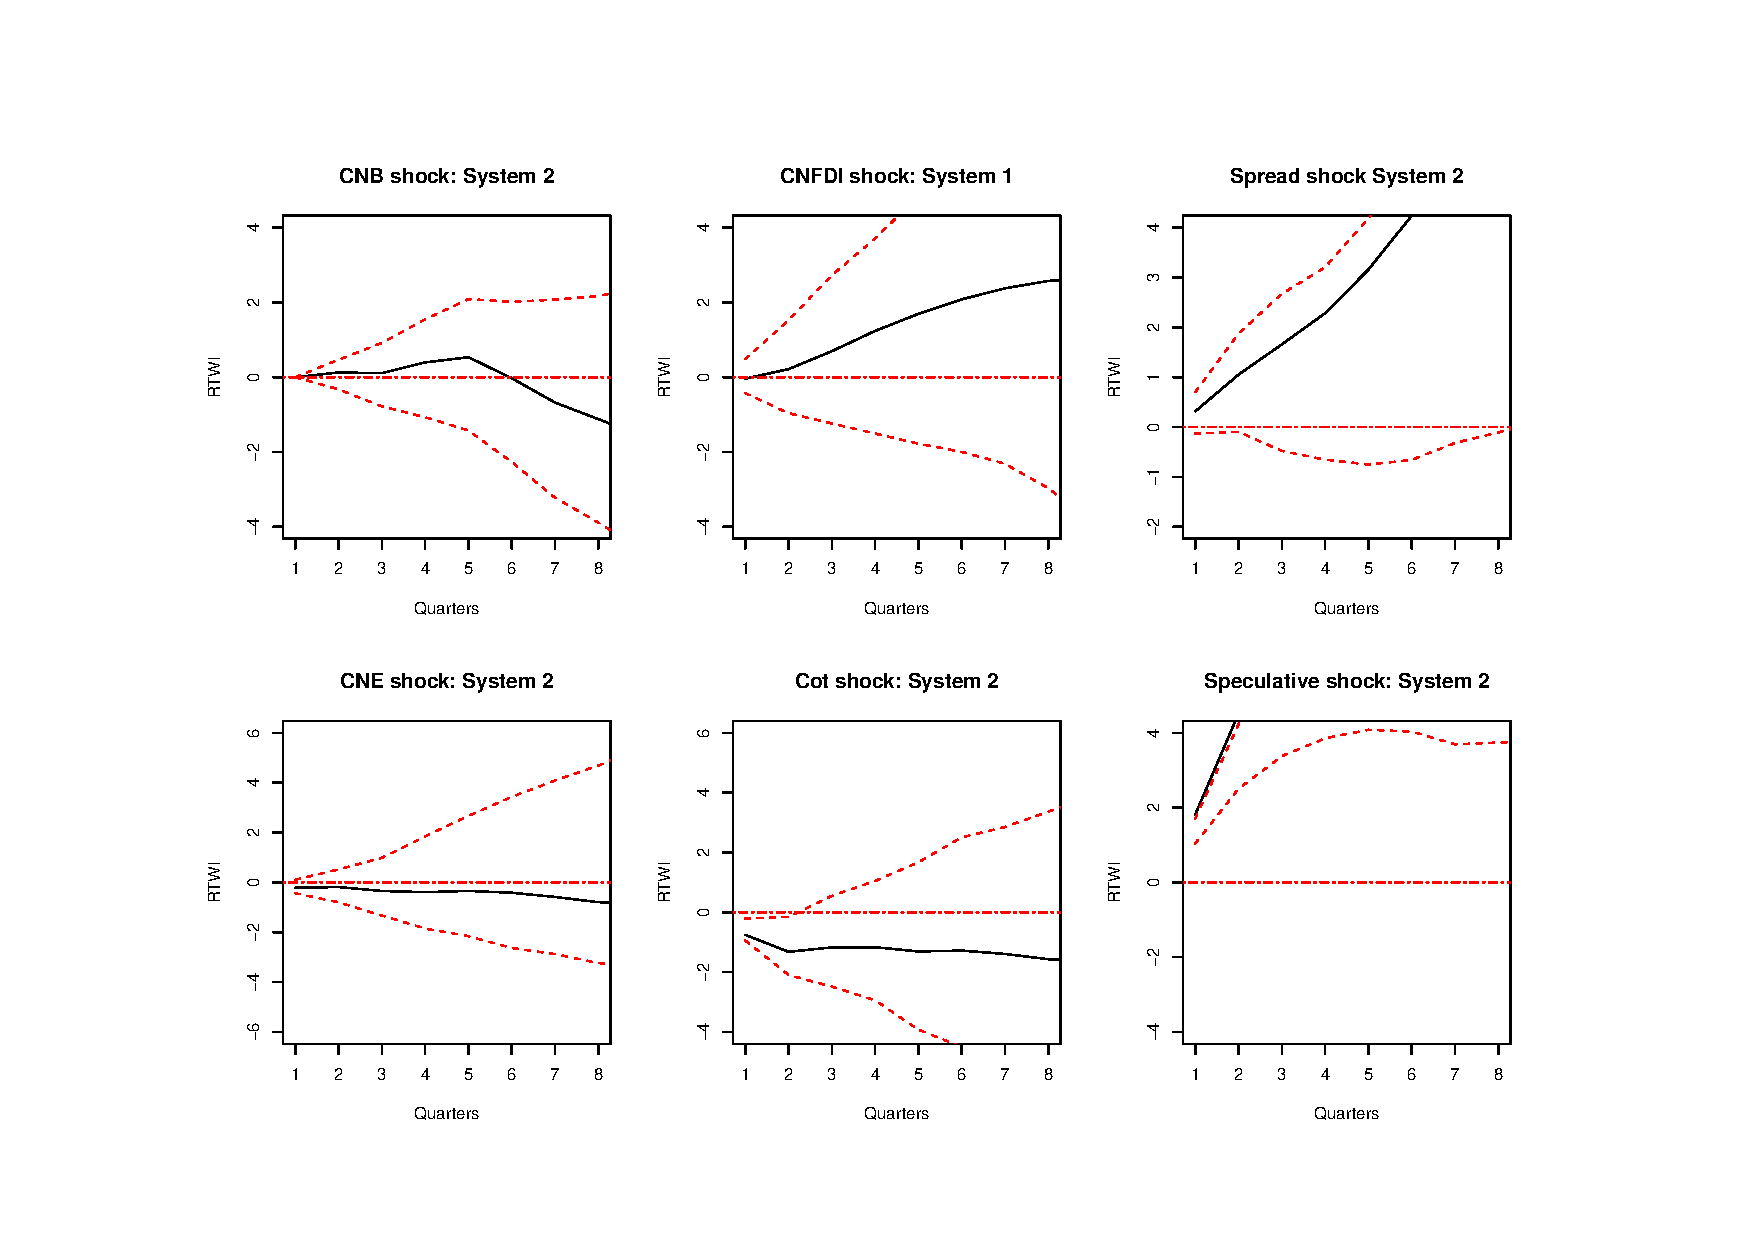
\includegraphics[scale=0.75]{IRF2}
\end{sidewaysfigure}

% does some additional infirmation about diagnositc tests (possibly with reference to appendix) come in here? 
It is encouraging that the broad patterns identified in the IRFs remain very similar no matter which of the three methods is used to identify the system (see Figures \ref{fig:IRF1}, \ref{fig:IRF2} and \ref{fig:IRF3} for IRFs from specifications One, Two and Three respectively).  The speculative effects related to sentiment and interest rate differentials are unequivocally positive in all three cases. The other major effect that is identified is that of the positive relationship between the official purchase of treasuries and the exchange rate.  The different methods of identifying the system all indicate that the other capital flows have a much more uncertain effect on the real exchange rate.  

The one difference that is evident in the IRF from the three different system is that for System One the initial impact of a positive shock to the purchase of bonds by foreign official institutions is negative and then turns positive in line with the other two systems.  This may be the result of reverse causation as it is most likely that the foreign exchange intervention will take place at times when the US dollar is weak. This is very plausible. 

\section{Conclusion}\label{secref:5}
An SVAR model of the real exchange rate and international capital flows is estimated and IRF are used to analyse the effect of shocks to the system.   Unlike most attempts to assess the relationship between capital flow and the exchange rate, this model includes a role for speculation. New methods have been proposed to measure speculative activity.  These measures seek to capture two types of speculation:  sentiment and the carry-trade.   
The IRFs that have been presented suggest that deviations from PPP can be explained by innovations in net international capital flows but, contrary to some of the other investigations of this issue, the type of flow that has the most pronounced and significant effect is that associated with speculation. This means that speculation is the key factor that is driving the exchange rate away from equilibrium and that speculation can affect competitiveness. Speculation can either flow from sentiment or carry-like positions.   

The results suggest that measures to reduce the effect of speculation can enhance economic stability.  In addition to the effect on competitiveness, these short-term capital flows can add liquidity to the banking system, fuel a credit book and cause an appreciation of asset prices.  These measures could be taxation or capital controls or intervention in the foreign exchange market.  There is some evidence that these direct interventions in the market can be effective. The other capital flow that has a consistent, positive and statistically significant effect on the real exchange rate associated with official intervention in the foreign exchange market. This provides evidence that official intervention in the foreign exchange market may be effective in offsetting some of the effect of speculative activity.  However, this paper does not assess the way that this intervention may affect other aspects of monetary policy. As such, capital controls or other forms of official activity may be more effective policy instruments against speculation in the medium to long term. 

%There has been only limited progress in the development of exchange rate models that depend on capital flows.  There have been three major problems in their contruction:  deciding on the variables that will be used, dealing with the issue of endogeneity and modelling the relationship between portfolio choice and the exchange rate.  This paper seeks to address these three issues. There is a discussion of the empirical evidence that underpins the relationship between capital flows and the exchange rate; there is at attempt to measures speculative flows; there is also a discussion of the effect of exchange rate intervention that does not depend on monetary changes or signalling.   There are three important contributions:  creating a structural model of international capita flows and the real exchange rate; adding speculation to the capital flows that are assessed; assessing the effect of speuclation in the model.   
%
\bibliography{../../myrefs}
\end{document}

\begin{appendices}
\section{Appendix 1}\label{app1}
\subsection{The data}
The current account data are taken from the US balance of payments that are released by the Bureau of Labor Statistics.   The data on capital flows are derived from a number of sources.  The first source is the US balance of payments data.  These data give a broad overview of the position of the US relative to other economies.  The series that explain the flow of foreign direct investment (FDI) come from the balance of payments data.  The net of private, direct investment in foreign-owned assets in the US and US assets abroad are combined.   Since January 1977, the US Treasury has released a monthly report providing significant detail about the changes in the holding of long-term securities amongst US and overseas investors. This report is part of a series of reports under the Treasury International Capital Department (commonly known as the TIC data).  See \citet[p. 29]{Siourounis2004Capital} and US Treasury \citet{TIC} for a comprehensive overview. \citet[p.18]{siourounis2004Capital} has a discussion of the way that share-swaps for overseas mergers may affect the data; \citet[p.516]{brookscapital} and \citet{HauEquity} discuss some of the limitations of the data and .

The data include information about the buying and selling of long-term securities by US and overseas investors.  From the gross figures for purchase and sale of specific securities by US-based and overseas investors, a net flow figure for each direction can be constructed for each security type by amalgamating gross purchase of overseas securities by US investors with the gross sale of US securities by overseas.  

\begin{equation}
NB= NUSB + NFB
\end{equation}

Where NB is net bonds; NUSB is net US bonds; NFB is net foreign bonds. 

\begin{equation}
NUSB = NT + NA + NC
\end{equation}

NT is net treasuries; NA is net agency securities; and, NC is net corporate bonds.  The net position is calculated by subtracting the gross sale of securities by overseas investors to US residents from the gross purchase of securities from overseas investors from US residents. 

\begin{equation}
NE = NUSE + NFE
\end{equation} 

Where NE is net equity; NUSE is net US equities; NFE is net foreign equities.  As before, the net position is the difference between gross purchase and gross sales by US residents.  

The other data that are available from the US Treasury are details on the transactions carried out by international monetary authorities.  These \emph{official} institutions are mostly central banks but can also include the IMF and other quasi-official organisations. By far the largest component of these are the purchase and sale of US Treasury bonds.  An increase in capital inflow to the US associated with official flows would be expected to come from pressure for appreciation of domestic currency vs the US dollar.  The most obvious example of  this is ``Mainland China" where the Chinese monetary authorities have acquired a huge holding of US Treasury bonds as they have bought US dollars against their own currency to maintain competitiveness \citet{TIC}.

The monthly official bond flow are subtracted from the total bond flows to leave a figure for the private sector and one for the pubic sector as well as a monthly series for net equity flows.  Once the three series  are added together to get quarterly figures they are placed with the current account and foreign direct investment flows (which came from the balance of payments) and all of these are cumulated from the starting point to get something approaching a stock of international assets and are then deflated by nominal GDP to facilitate the comparison across time. 

The first speculative money market series are compiled to account for sentiment, momentum or technical tracing flows.  The series for these flows are the positions held by speculative funds in the main currency futures markets in the US.  These are positions that must be reported to the US derivative regulator, the US Commodity Futures Trading Commission (CFTC).  The positions are held in foreign currency vs the US dollar.  The key contracts are Canadian Dollar (contract of 100,000 Canadian dollars), UK Sterling (contract of 62,500 sterling), Japanese yen (12,500,000 yen), Swiss franc (125,000 CHF) and Euro (125,000 EUR) or Deutschmark before the introduction of ECU trading.  The data and explanation about the differentiation between commercial (hedgers) and non-commercial (speculators) is available from the CFTC web site \citet{cot}.   The outstanding long or short speculative positions are amalgamated across currencies and normalised to the total number of speculative positions (S1) or the total open interest positions (S2) to get an overall measure of sentiment.  Once the two series are constructed, they are multiplied by -10 to make something easier to work with and to ensure that a speculative inflow to the US is a positive number. 

The interest rate data are taken from the IMF International Financial Statistics.  The interest rates are short-term interest rates and usually 'money market rates' where available.  The three month rate is used. An index of international money rates is compiled and compared to the equivalent US interest rate. The index is composed with weights equal to those used in the Major Currency trade-weighted index that is compiled by the US Federal Reserve \citet{Fedtwi}.  For the Euro, an equal weight of French and German rates is taken until the arrival of the ECU.   Mexico causes some problems as it has a relatively large trade weight with the US and, in the 1980s, had very volatile interest rates.  This means that the interest rate spread is quite volatile in the early years of the series.  Therefore, there are two spread series created.  The first (SPREAD1) includes Mexico and the second (SPREAD2) excludes Mexico.  In the VAR analysis, a dummy variable is also used to account for the interest rate volatility in the early 1980s.    

\subsection{Data preparation}
Therefore, there are seven main variables that are to be used in the analysis and a number of variations that can be applied to the model.  The main variables are: the cumulative current account balance per GDP (CCA); the cumulative net bond per GDP (CNB); the cumulative net equity per GDP (CNE); cumulative net foreign direct investment per GDP (CNFDI); cumulative net official treasuries per GDP (COT); the real trade-weighted index (RTWI); and the nominal trade-weighted index (NTWI); the spread between US short rates and the rates of the main trading partners (SPREAD1 includes Mexico and SPREAD2 does not); and, a measure of speculative sentiment measured in two ways (S1 and S2).  The full data set run from the first quarter of 1973 through to the first quarter of 2010.  However, the series taken from the Transactions in Long Term Securities data (TIC) only begin in the second quarter of 1977, the data on official holdings of US Treasury bonds begin in the second quarter of 1978 and the sentiment data begin in the first quarter of 1986.   
\begin{sidewaystable}
%this comes from the R file.  
%pdflandscape is required to facilitate the landscape position. 
% latex table generated in R 2.15.0 by xtable 1.7-0 package
% Sun Jun 10 12:46:12 2012
\begin{threeparttable}
\caption{Important capital flows and exchange rate data}
\begin{tabular}{p{4cm}rrrrrrrrrrr}  
   \hline
 & CCA & DCCA & CNB & CNE & CNFDI & COT & RTWI & SPREAD & S1 & S2 \\ 
  \hline
Q1 2007  & -179.02 & -5.22 & 12.92 & -0.55 & -2.99 & 0.71 & 89.89 & 2.63 & -0.08 & -0.12 \\ 
Q2 2007  & -181.66 & -5.44 & 13.80 & 2.37 & -3.27 & 0.28 & 87.68 & 2.38 & 0.02 & 0.02 \\ 
Q3 2007  & -184.95 & -5.21 & 7.67 & 0.27 & -3.21 & -0.31 & 85.45 & 2.00 & 0.14 & 0.23 \\ 
Q4 2007 & -187.92 & -4.62 & 5.45 & 0.49 & -5.32 & -0.19 & 81.58 & 1.46 & 0.21 & 0.33 \\ 
Q1 2008  & -191.90 & -4.25 & 9.53 & 2.55 & -6.07 & 2.13 & 80.40 & 0.42 & 0.15 & 0.25 \\ 
Q2 2008  & -194.88 & -4.87 & 11.26 & -0.17 & -6.19 & 2.23 & 79.34 & -0.57 & 0.04 & 0.07 \\ 
Q3 2008  & -200.48 & -5.32 & 8.52 & 0.22 & -6.51 & 1.10 & 82.82 & -0.73 & -0.08 & -0.14 \\ 
Q4 2008  & -209.21 & -4.26 & 0.52 & 2.02 & -6.03 & -0.11 & 90.14 & -0.99 & -0.08 & -0.15 \\ 
Q1 2009 & -214.35 & -2.31 & -0.36 & 1.92 & -7.46 & 0.04 & 91.40 & -0.63 & -0.08 & -0.14 \\ 
Q2 2009  & -217.36 & -2.40 & 3.24 & 0.74 & -8.45 & 1.24 & 88.12 & -0.50 & -0.03 & -0.06 \\ 
Q3 2009  & -219.53 & -3.21 & 4.07 & 1.13 & -9.21 & 1.89 & 84.08 & -0.52 & 0.16 & 0.25 \\ 
Q4 2009 & -219.87 & -2.94 & 6.70 & 1.93 & -9.83 & 3.36 & 81.46 & -0.57 & 0.12 & 0.19 \\ 
Q1 2010 & -219.52 & -2.58 & 9.95 & 1.58 & -11.48 & 2.82 & 83.65 & -0.56 & -0.10 & -0.16 \\ 
   \hline
\label{tab:capflow}
\end{tabular}
\begin{tablenotes}
\small
\item These are the data that are used in the analysis.   CCA is the cumulative current account normalised by GDP; DCCA is the change in the cumulative current account; CNB is the cumulative net bond position per GDP; CNE is the cumulative net equity position per GDP; CNFDI is the cumulative net flow of foreign direct investment per GDP; COT is cumulative official treasuries purchase per GDP; RTWI is the real trade-weighted index of major currencies; SPREAD is the spread between US 3 month LIBOR and a basket of equivalent overseas rates (the same currencies as the trade-weighted index); S1 and S2 are indexes of speculative sentiment based on the average speculative positions disclosed to the CFTC by buyers of currency futures relative to the US dollar (Japanese yen, Swiss Franc, Euro or Deutschemark and Pound Sterling).  S1 is the net position of speculators relative to speculative positions; S2 is the net position of speculators relative to the open interest (total of all outstanding open positions).  A positive number is a US asset, an appreciation of the exchange rate, a US interest rate advantage or speculation in favour of the US dollar. 
\end{tablenotes}
\end{threeparttable}  
\end{sidewaystable}
\section{Appendix 2}\label{app2}
What goes in here?  Diagnostic tests and table for the different models? 
The FDI data come from the US balance of payments, net portfolio flows are from the US Treasury International Capital data, speculative momentum is based on CFTC speculative positions and the interest rate differential is a proxy for the carry-trade. Fuller details of the variables.   

\end{appendices}
\end{document}
